\documentclass{beamer}
\usepackage[utf8]{inputenc}

\usetheme{Madrid}
\usecolortheme{default}
\usepackage{amsmath,amssymb,amsfonts,amsthm}
\usepackage{txfonts}
\usepackage{tkz-euclide}
\usepackage{listings}
\usepackage{adjustbox}
\usepackage{array}
\usepackage{tabularx}
\usepackage{gvv}
\usepackage{lmodern}
\usepackage{circuitikz}
\usepackage{tikz}
\usepackage{graphicx}

\setbeamertemplate{page number in head/foot}[totalframenumber]

\usepackage{tcolorbox}
\tcbuselibrary{minted,breakable,xparse,skins}

% Code styling
\lstset{
    language=C,
    basicstyle=\ttfamily\small,
    keywordstyle=\color{blue},
    stringstyle=\color{orange},
    commentstyle=\color{green!60!black},
    numbers=left,
    numberstyle=\tiny\color{gray},
    breaklines=true,
    showstringspaces=false,
}
%------------------------------------------------------------

\title
{2.6.14}
\date{September 14, 2025}
\author 
{AI25BTECH11008\\Chiruvella Harshith Sharan}

\begin{document}

\frame{\titlepage}

\begin{frame}{Question}
\begin{center}
Find the area of the parallelogram whose diagonals are
\[
\vec{d_1} = 2\hat{i} - \hat{j} + \hat{k}, \quad
\vec{d_2} = \hat{i} + 3\hat{j} - \hat{k}.
\]
\end{center}
\end{frame}

% Step 1
\begin{frame}{Diagonals}
\begin{center}
The diagonals are
\[
\vec{d_1} = \begin{bmatrix}2 \\ -1 \\ 1\end{bmatrix}, \quad
\vec{d_2} = \begin{bmatrix}1 \\ 3 \\ -1\end{bmatrix}.
\]
The area of the parallelogram is given by
\begin{equation}
A = \tfrac{1}{2}\|\vec{d_1} \times \vec{d_2}\|.
\end{equation}
\end{center}
\end{frame}

% Step 2
\begin{frame}{Cross Product}
\begin{center}
Computing the cross product:
\begin{equation}
\vec{d_1} \times \vec{d_2} =
\begin{vmatrix}
\hat{i} & \hat{j} & \hat{k} \\
2 & -1 & 1 \\
1 & 3 & -1
\end{vmatrix}
= \begin{bmatrix}-2 \\ 3 \\ 7\end{bmatrix}.
\end{equation}
\end{center}
\end{frame}

% Step 3
\begin{frame}{Magnitude}
\begin{center}
The magnitude is
\begin{equation}
\|\vec{d_1} \times \vec{d_2}\| = \sqrt{(-2)^2 + 3^2 + 7^2}
= \sqrt{62}.
\end{equation}
Hence,
\begin{equation}
A = \frac{\sqrt{62}}{2}.
\end{equation}
\end{center}
\end{frame}


% ------------------- C Code -------------------
\begin{frame}[fragile]
    \frametitle{C Code}
    \begin{lstlisting}
#include <stdio.h>
#include <math.h>

int main() {
    // Define diagonals as vectors
    int d1[3] = {2, -1, 1};
    int d2[3] = {1, 3, -1};

    // Cross product d1 x d2
    int cross[3];
    cross[0] = d1[1]*d2[2] - d1[2]*d2[1]; // y1*z2 - z1*y2
    cross[1] = d1[2]*d2[0] - d1[0]*d2[2]; // z1*x2 - x1*z2
    cross[2] = d1[0]*d2[1] - d1[1]*d2[0]; // x1*y2 - y1*x2

    // Magnitude of cross product
    double mag = sqrt(cross[0]*cross[0] + cross[1]*cross[1] + cross[2]*cross[2]);

    \end{lstlisting}
\end{frame}

\begin{frame}[fragile]
    \frametitle{C Code}
    \begin{lstlisting}

    // Area of parallelogram
    double area = 0.5 * mag;

    // Output result
    printf("Area of the parallelogram = %lf\n", area);

    return 0;
}

    \end{lstlisting}
\end{frame}

\begin{frame}[fragile]
    \frametitle{Python Code}
    \begin{lstlisting}
    
import numpy as np
import matplotlib.pyplot as plt

# Define diagonals as numpy arrays
d1 = np.array([2, -1, 1])
d2 = np.array([1, 3, -1])

# Diagonal endpoints (parallelogram diagonals intersect at the origin)
A = -0.5 * d1
B = 0.5 * d1
C = -0.5 * d2
D = 0.5 * d2


    \end{lstlisting}
\end{frame}

% ------------------- Python Plot -------------------
\begin{frame}[fragile]
    \frametitle{Python Code}
    \begin{lstlisting}
# Parallelogram vertices: A+C, A+D, B+D, B+C
P1 = A + C
P2 = A + D
P3 = B + D
P4 = B + C

# Collect vertices for plotting closed shape
parallelogram = np.array([P1, P2, P3, P4, P1])

# 3D plot
fig = plt.figure(figsize=(6,6))
ax = fig.add_subplot(111, projection='3d')

# Plot parallelogram edges
ax.plot(parallelogram[:,0], parallelogram[:,1], parallelogram[:,2], 'b-', label="Parallelogram")


    \end{lstlisting}
\end{frame}

\begin{frame}[fragile]
    \frametitle{Python Code}
    \begin{lstlisting}
    
# Fill parallelogram face
ax.plot_trisurf(parallelogram[:,0], parallelogram[:,1], parallelogram[:,2], color='cyan', alpha=0.5)

# Plot diagonals
ax.plot([A[0], B[0]], [A[1], B[1]], [A[2], B[2]], 'r--', label="d1")
ax.plot([C[0], D[0]], [C[1], D[1]], [C[2], D[2]], 'g--', label="d2")

# Labels and legend
ax.set_xlabel('X')
ax.set_ylabel('Y')
ax.set_zlabel('Z')
ax.set_title('Parallelogram with diagonals d1 and d2')
ax.legend()

plt.show()

    \end{lstlisting}
\end{frame}

\begin{frame}{Plot}
   \centering
   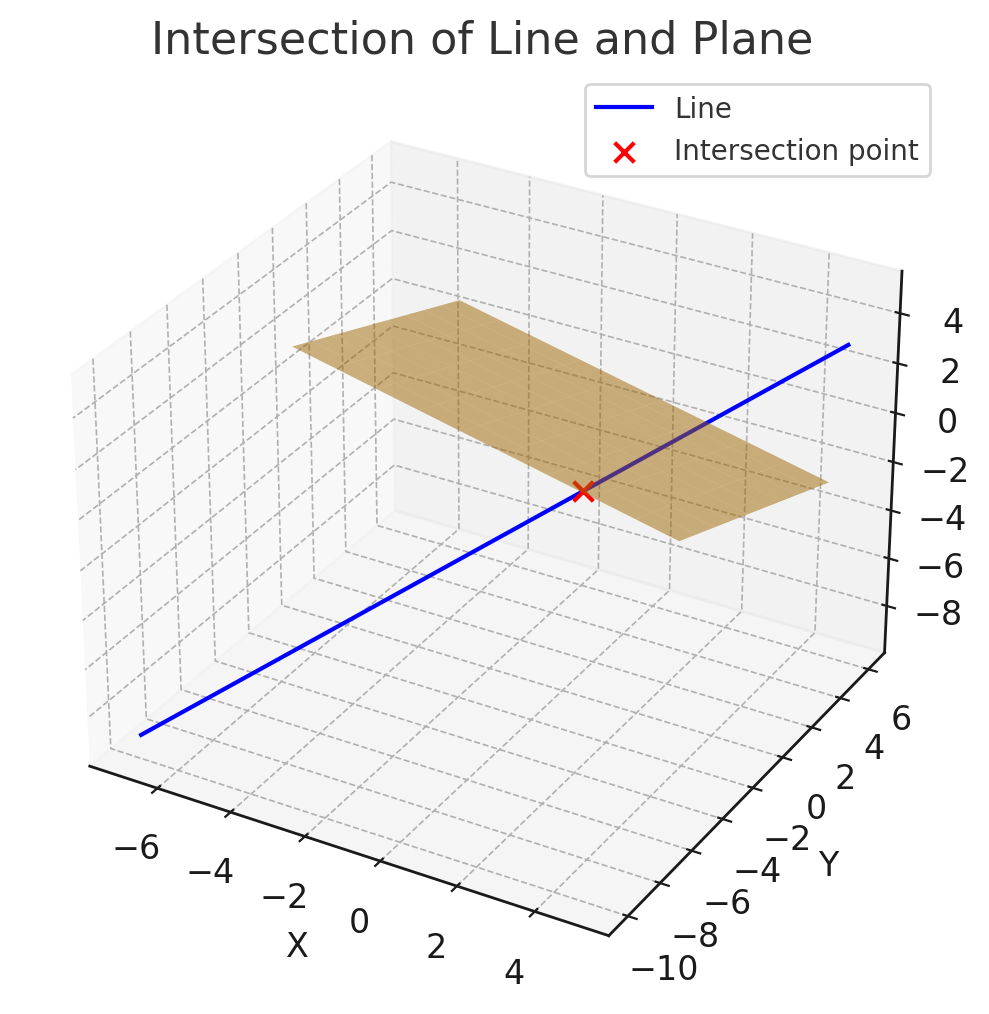
\includegraphics[width=\columnwidth, height=0.8\textheight, keepaspectratio]{beamer/figs/fig1.jpg}
   \label{fig:Beamer/figs/fig1.png}
\end{frame}

\end{document}
